\chapter{Implementação do Sistema} \label{cap:implementacao}

Este sistema, por ser desenvolvido na plataforma Outsystems, é constituído por módulos, que representam os vários elementos do sistema.\\
O módulo onde será desenvolvido o servidor e a interface para os utilizadores é o módulo WaterWatcher. O módulo que servirá para manter os dados será o WaterWatcherService.\\
Por fim desenvolvemos também um módulo de testes (WaterWatcherTests) e um módulo que simula as interações com o sistema informático da empresa fornecedora de água, denominado SimulCompany.
Este capítulo tem como propósito clarificar e justificar as várias decisões que tomámos no desenvolvimento dos vários módulos do projeto.\\
Na secção \ref{modww} vamos abordar o módulo WaterWatcher, na secção \ref{modwws} o módulo WaterWatcherService e na secção \ref{modsc} o módulo que simula o sistema da companhia fornecedora de água.\\


\section{Módulo WaterWatcher} \label{modww} %Water Watcher-----------------------------------------------
Este módulo é onde serão desenvolvidos a aplicação para os utilizadores e a lógica do servidor. Sendo assim, este módulo está dependente dos módulos WaterWatcherService e SimulCompany, sendo estas as únicas dependências entre os módulos do projeto.\\
Decidimos implementar a aplicação e o servidor no mesmo módulo dado que a plataforma nos permite implementar ações específicas do servidor ou do cliente num mesmo módulo, podendo distinguir quais os processos que irão ser executados nos servidores da aplicação ou no dispositivo dos clientes sem ser necessário criar mais estruturas de código.\\
Este módulo implementa toda a lógica e as vistas da aplicação para os utilizadores.

\section{Módulo WaterWatcherService} \label{modwws} %Water Watcher Service------------------------------
Este módulo é onde implementamos toda a lógica relativa ao armazenamento de informações que vamos utilizar neste sistema. No diagrama [ adicionar diagrama] podemos observar uma representação gráfica das várias entidades que armazenamos.\\
Os clientes têm os todos os atributos propostos na secção \ref{sec:dados} e têm ainda um atributo único que os identifica denominado idUser, que é gerado automaticamente aquando da criação de um novo utilizador. Este identificador é também o identificador de outra estrutura, que é a estrutura User. Esta estrutura contém as mesmas informações da estrutura Cliente, porém como esta é uma estrutura em qual a autenticação em aplicações construídas nesta plataforma se baseia \cite{outs:users} não poderíamos substituí-la.

\section{Módulo SimulCompany} \label{modsc} %Simul Company------------------------------
O módulo SimulCompany é o elemento do projeto que simula o sistema informático da empresa fornecedora de água, de forma a podermos testar o nosso sistema. Por não termos acesso ou conhecimento sobre o sistema informático das várias empresas de água que poderão utilizar o nosso sistema, decidimos implementar um sistema apenas com um elemento de armazenamento de dados e algumas funções simples de acesso e modificação desses dados, para que o sistema Water Watcher possa funcionar com o máximo de interfaces programáticas possíveis, dado que não requer muitas funcionalidades e operações do sistema com o qual vai comunicar.\\
Os dados deste módulo possuem vários atributos e relações que estão representados de forma gráfica na figura.

[adicionar figura]

Como podemos observar na figura, a entidade Cliente representa um cliente do serviço de fornecimento de água, sendo ele identificado unicamente pelo seu número de cliente. Também terá outros atributos associados que são necessários para a sua identificação ou de forma a poder ser contactado como o número de conta, nome, email e o contacto telefónico.\\ 
Cada cliente terá associados um ou mais Contadores, identificados unicamente pelo seu número de Instalação. São também armazenados o número de série e o contrato e o cliente aos quais o contador está associado.\\
Existe também a entidade Contagens que representa uma contagem mensal de um contador, que é composta por um identificador único, o mês e ano em que foi emitida, o preço que o cliente pagou, a medição do contador na altura da contagem, a diferença para o mês anterior e o contador associado a essa contagem.\\
Por fim, criámos a entidade Localização que estará associada aos clientes e aos contadores representando, respetivamente, a morada do cliente e o local onde o contador está implementado. Uma localização é composta por um identificador único, rua, localidade, freguesia, concelho, distrito e país.\\ 
Neste módulo estão implementadas também as funções que permitem aceder, modificar e apagar as instâncias criadas das entidades. Para além destas operações, implementámos também uma função que nos permite saber quais os contadores de um cliente que não tiveram uma contagem submetida para o mês atual, e algumas funções que envolvem mais do que uma entidade, como obter as contagens de um cliente num intervalo de anos.


\section{Ecrãs de Log in e Registo} \label{ecra:login} %ECRA Login #####################################
A primeira página com a qual o utilizador interage é a página de log in. Esta página, para além de apresentar os contactos da empresa fornecedora, permite que o utilizador se registe ou se autentique com a sua conta já existente.
O registo no sistema segue o processo representado na figura \ref{fig:registo}.

\begin{figure}[h!]
\begin{center}
\resizebox{120mm}{!}{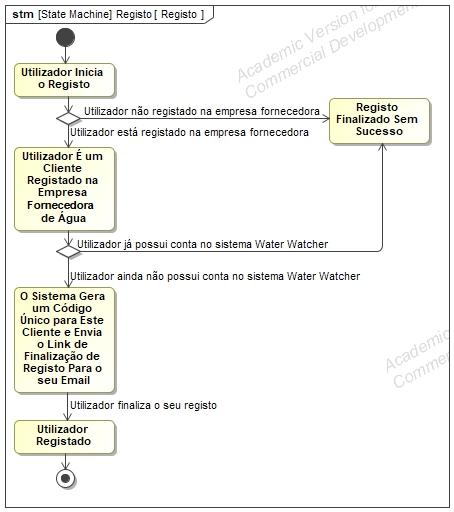
\includegraphics{diagramas/svg/Registo.jpg}}
\caption{Processo de registo no sistema.}
\label{fig:registo}
\end{center}
\end{figure}

Como descrito na figura, após o utilizador iniciar o registo e indicar o seu número de cliente, o sistema verifica se existe algum cliente registado na empresa fornecedora com esse número de cliente. Caso não exista nenhum cliente, é apresentada uma mensagem de erro. Se existir, o sistema verifica agora se este cliente já se encontra registado no serviço. Caso já se encontre registado, não será possível criar uma nova conta para este cliente, sendo assim apresentada uma nova mensagem de erro.\\
Sabendo agora que o cliente existe e não tem conta no sistema, é enviado um link para o email associado à conta do cliente no sistema da empresa fornecedora de água. Este link contém um código gerado aleatoriamente que permitirá ao utilizador finalizar o seu registo, definindo uma palavra-passe. Após este registo, o sistema obtém as informações deste cliente na empresa fornecedora e é então gerado um novo utilizador no sistema .\\
Para a geração deste código aleatório, recorremos à biblioteca RNGCryptoServiceProvider \cite{RNGCryptoServiceProvider} onde geramos um código de 20 caracteres (letras maiúsculas, minúsculas e números). Ao início deste código vai ser adicionado o número de cliente seguido por um ‘.’ , para que possamos identificar o cliente ao qual o código está associado apenas pelo código em si. Este código é depois apagado do sistema após o registo do cliente.\\
Depois de registado o utilizador poderá fazer o log in, indicando o seu número de cliente e a palavra-passe que definiu. 

\section{Ecrã de Informações e Estatísticas} \label{ecra:info} %ECRA Info ##################################
No ecrã de informações e estatísticas o cliente pode consultar as suas contagens de forma gráfica e os detalhes das suas faturas para os seus vários contadores e em diferentes anos.\\
Caso esteja inscrito no programa de controlo semanal também poderá visualizar as suas várias contagens semanais de forma gráfica para os vários contadores, anos e meses.\\
Por não mantermos um registo das faturas mensais dos utilizadores na base de dados do sistema, estas são obtidas através de pedidos ao sistema informático da empresa fornecedora.\\
De forma a não fazer pedidos em excesso a esse sistema informático, quando o utilizador carrega a página, serão carregadas as suas faturas para o ano atual e o ano passado. Posteriormente, caso o utilizador selecione outro ano para obter as faturas, é feito um novo pedido à empresa, porém essas faturas ficam guardadas localmente para que não sejam feitos novos pedidos à empresa cada vez que o utilizador seleciona esse ano nessa mesma sessão de utilização. Ou seja, só é feito um pedido à empresa da primeira vez que o utilizador seleciona esse ano e contador nessa sessão.\\

\section{Ecrã de Definições} \label{ecra:def} %ECRA Definic #####################################
No ecrã de definições, são apresentadas ao cliente as informações relacionadas com a sua conta na empresa fornecedora de água, mais concretamente, o seu número de cliente, número de conta, nome, email e telefone.\\
O cliente poderá também alterar o seu email e telefone, sendo que esta informação será alterada neste sistema informático e no da empresa de água.\\
O cliente também poderá atualizar as suas informações, ou seja, caso tenha sido alterada alguma informação da sua conta na empresa, o cliente poderá atualizar a sua informação no sistema, sendo verificada e alterada a sua informação neste sistema informático, de acordo com a informação presente no sistema da empresa, de forma esta que fique consistente em ambos.

\section{Ecrã de Envio de Leituras} \label{ecra:leituras}  %ECRA OCR #####################################
Esta página permite aos clientes do serviço enviar as suas contagens mensais e semanais, caso esteja inscrito no programa de controlo semanal.\\
O envio das contagens só é possível durante alguns dias, sendo eles o dia escolhido para o envio das contagens semanais e o dia seguinte, e os dias finais de cada mês para o envio das contagens mensais. Atualmente o dia definido para o início do envio das contagens mensais é o dia 25 de cada mês, porém este dia pode ser alterado.\\
Também é possível, nesta página, que o cliente se inscreva, ou desista do programa de controlo semanal de contagens. Para a inscrição apenas precisa de selecionar o dia de semana e hora a que pretende ser notificado e após finalizar a inscrição será relembrado semanalmente no tempo escolhido através de um email.\\
Por fim, o envio da contagem pode ser feito por texto, escrevendo a leitura atual do contador, ou através de uma fotografia, que encaminhará o utilizador para o ecrã de envio da fotografia.\\
Para ambos os casos, deverá ser selecionado o contador em questão, de entre os contadores apresentados numa caixa de seleção. Apenas são apresentados os contadores que ainda não têm contagem submetida no determinado mês ou semana.

\section{Ecrã de Envio de Fotografia do Contador} \label{ecra:foto}  %ECRA Foto #############################
Quando o utilizador inicia o processo de envio da fotografia do seu contador, a câmara do seu dispositivo é ativada e o ecrã passa a transmitir o que a câmara está a captar, aparecendo no centro do ecrã uma moldura retangular azul. O utilizador deve alinhar os algarismos que mostram a leitura (com fundo preto) com a moldura, como representado na figura \ref{fig:moldura}, dado que o sistema vai apenas recolher a imagem que está contida nessa moldura.\\
Posteriormente, a aplicação móvel envia a imagem para o servidor, local onde será feito o OCR.\\
Após o utilizador fotografar o contador, é efetuada a seleção da porção da fotografia dentro dos limites da moldura. Depois, transformamos a imagem num array de byte, utilizando o método \textit{toDataUrl} , que nos permite obter a imagem no esquema Data Uri \cite{dataurl}, em que temos um campo que contém a imagem codificada em base64. Acedendo à propriedade \textit{src} deste elemento podemos verificar que o array obtido representa, de facto, a secção da fotografia pretendida.\\
Posteriormente convertemos esse array de base 64 em um array de bit, que é a forma definida nesta plataforma para guardar imagens.

\begin{figure}[h!]
\begin{center}
\resizebox{120mm}{!}{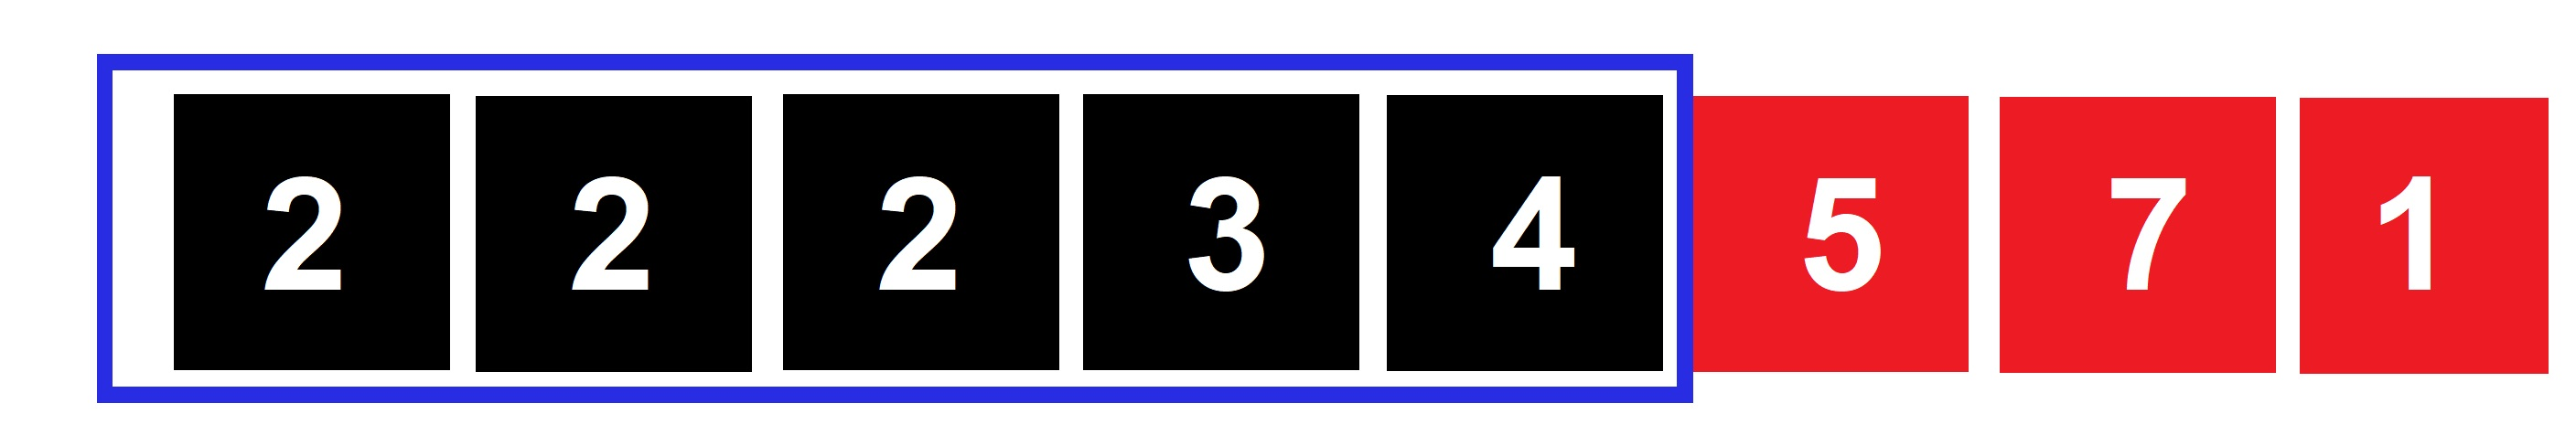
\includegraphics{diagramas/moldura.jpg}}
\caption{Esquematização do alinhamento da moldura com os caracteres da medição de água.}
\label{fig:moldura}
\end{center}
\end{figure}

Depois de o servidor efetuar o OCR, é enviado para a aplicação cliente o resultado desta operação e um número compreendido entre 0 e 100 que representa a confiança no resultado, ou seja, a probabilidade calculada pelo módulo de OCR de o resultado estar correto.\\
Caso a confiança seja menor de 65, é apresentado ao utilizador uma mensagem de erro de forma a que o utilizador envie uma nova fotografia.\\
Se for maior ou igual a 65, é apresentado ao utilizador o texto obtido para que este possa confirmar se este está correto e, nesse caso, submeter a sua leitura ou para que este possa enviar uma nova fotografia.\\
Durante a submissão da leitura, no servidor, é verificado se o contador relativo à contagem enviada, que é passado como parâmetro \textit{query string}, pertence ao utilizador que está a enviar o pedido.

\section{Ecrã de Administração} \label{ecra:admin} %ECRA Admin #####################################
A página para os administradores permite a utilizadores com papeis de administração notificar utilizadores sob a forma de email, bem como apagar utilizadores da base de dados do sistema.\\
A notificação de utilizadores inicia-se quando o utilizador seleciona o destinatário da mensagem, que pode ser um utilizador em específico, identificado pelo seu número de cliente, todos os utilizadores registados cuja morada se encontre na freguesia indicada ou todos os utilizadores do sistema.\\
Como referido anteriormente, este utilizador também poderá apagar outros utilizadores da base de dados do sistema, apenas indicando o número de cliente do utilizador a apagar. Esta ação apaga as contagens semanais, os seus contadores e a sua informação pessoal na base de dados do sistema.


\section{Módulo de Testes WaterWatcherTests} \label{ecra:admin} %MODULO Tests ###############################

Para o desenvolvimento de testes unitários aos componentes desenvolvidos, elaborámos um módulo de testes também na plataforma Outsystems.\\
Este módulo está desenvolvido segundo a metodologia BDD (Behavior Driven Development) \cite{bddtests}, ou seja, desenvolver testes que replicam o comportamento de um utilizador na aplicação, testando as funções e processos envolvidos nessas ações e ao mesmo tempo descrevendo textualmente o que é que está a ocorrer.\\
Esta aplicação possuí uma interface gráfica que nos permite observar o resultado dos cenários de teste e das ações que os compõem. Esta interface gráfica é composta por duas páginas: a página que apresenta os resultados dos testes e uma página de testes ao reconhecimento de caracteres.\\
Cada teste individual a uma funcionalidade da aplicação, denominado de cenário, é composto por vários passos que se encaixam em uma de três fases do teste. A primeira fase (Given) descreve o contexto do sistema aquando do início do teste e configura o sistema para o estado pretendido para que possamos começar o teste. A segunda fase (When) descreve um evento ou interação com o sistema, que pode ser iniciada por um utilizador ou outro sistema. A terceira e última fase (Then) é quando comparamos o resultado obtido com o resultado expectado.\\
A página de teste ao OCR permite-nos submeter imagens para a deteção de caracteres e observar o resultado e confiança obtidos.














